\chapter{Fundamentos básicos}

Este capitulo apresenta os principais conceitos e definições necessários para o entendimento deste trabalho. A seção 2.1 apresenta alguns conceitos básicos em~\emph{Unified Modeling Language} (UML), que são necessários para o entendimento da modelagem deste trabalho.
A seção 2.2 disserta sobre conceitos a respeito da informática na educação.
A seção 2.3 aborda a teoria sobre Sistemas Multiagentes necessária para este trabalho.
A seção 2.4 contém a metodologia~\emph{Multiagent System Engineering}, desenvolvida para a criação de Sistemas Multiagentes
A seção 2.5 e 2.6 abordam o funcionamento dos frameworks JADE e Jboss Seam, respectivamente.
Por fim, a seção 2.7 detalha alguns trabalhos correlatos.

\section{Informática na Educação}
O uso do computador como meio de educação tornou-se essêncial atualmente. Popularizando meios que, antigamente, eram muito caros ou raros, a aquisição de conhecimento tornou-se muito simples bastando um computador com acesso a internet para o acesso à diversos tipos de conhecimento.

O computador passa então a ser uma forma de ensino, ocasionando na descentralização da figura do professor neste processo e, segundo~\cite{de2009}, promove o desenvolvimento cognitivo por meio de uma interação maior entre o aluno e o objeto de conhecimento.

Dessa forma a Informática na Educação (IE) constitui-se um importante ramo de estudo.

Com o crescimento da internet, surgem ambientes específicos para aplicações interativas que auxiliam o estudante. Estes ambientes, chamados de Ambientes Virtuais de Aprendizagem (AVA), surgiram na década de 90 com os cursos a distância e mais tarde com ferramentas interativas e em tempo real~\cite{penterich2005ambientes}.

Da necessidade em organizar as informações geradas pelos AVA, surgiram os Sistemas Gerenciadores de Conteúdo e Aprendizagem (LCMS –~\emph{Learning and Content Managment System}).

A interação entre as ferramentas tornou-se cada vez maior e tornou-se  cada vez mais necessário o ensino personalizado à cada estudante. A personalização está relacionada com a forma específica que cada estudante tem ao lidar com informações, a melhor forma de aprender, as suas habilidades. Entre outras palavras, os Sistemas começaram a interagir mais com os alunos a fim de determinar a forma como os alunos percebem e processam as informações.

\subsection{Estilo de Aprendizagem}
O estilo de aprendizagem é a forma mais eficiente em que o estudante absorve conhecimento ao receber e processar uma informação. Um modelo de estilo de aprendizagem visa classificar um estudante de acordo com uma escala que, organiza as formas as quais são possíveis receber e processar o conhecimento~\cite{felder1988learning}. Estilos de aprendizagem não classificam em uma escala melhor ou pior do que outro estilo de aprendizagem, apenas categoriza o aluno de acordo com a forma de aprender.

O estilo de aprendizagem pode orientar melhor um docente a estimular um aluno durante o processo de desenvolvimento de suas habilidades, alterando o ambiente para o aluno de acordo com o estilo de forma a individualizar o processo didádico do ensino. Existem diversos modelos de estilos de aprendizagem propostos na literatura.

\subsubsection{Modelo de~\emph{Kolb}}

A teoria de~\emph{Kolb} propõe uma perspectiva chamada de teoria experimental do aprendizado, pois enfatiza o fato da experiência no processo de aprendizagem. Kolb inicialmente baseia-se em um ciclo de aprendizado de quatro estágios: Experiência Concreta, observação reflexiva, conceituação abstrata e experimentação ativa. Basicamente o ciclo funciona de forma à iniciar nas experiências concretas prover fundamentos para o ciclo da observação reflexiva. A partir de observações e reflexões, novos conceitos abstratos são formados. Esses conceitos podem implicar em ações que podem ser colocadas em prática, criando assim novas experiências.

Os estilos de aprendizagem são combinados com o ciclo de aprendizado e são separados~\ref{lista_estilos_aprendizagem} em quatro categorias~\cite{kolb84}:

\begin{table}
	\caption{Estilos de Aprendizagem definidos por Kolb}
	\begin{tabular}{|p{4cm} | p{3cm} | p{7cm} |}
		\hline
		\textbf{Estilo de Aprendizagem}	& \textbf{Ciclos} & \textbf{Descrição}	\\
		\hline
		Divergente	& Experiência Concreta, Observação Reflexiva & Pessoas que utilizam a imaginação com mais facilidade para resolver problemas. São capazes de olhar um problema por diferentes perspectivas. Possuem maior interesse cultural e prazer pelo ganho da informação. 	\\
		\hline
		Assimilador	& Conceituação Abstrata, Observação Reflexiva & Possuem uma aproximação maior de raciocínio lógico, onde há ênfase em idéias e conceitos. São menos focadas em pessoas e mais focadas em conceitos abstratos. Valorizam mais as explicações detalhadas do que uma oportunidade prática. 	\\
		\hline
		Convergente	& Conceituação Abstrata, Experimentação Ativa & Possuem inclinação maior á situações práticas, onde utilizarão o seu conhecimento para resolver um problema de forma experimental.	\\
		\hline
		Acomodador	& Experiência Concreta, Experimentação Ativa & Usam-se de outras pessoas para suas análises, confiando em experiências de terceiros para tirar suas próprias conclusões.	\\
		\hline
	\end{tabular}
	\label{lista_estilos_aprendizagem}
\end{table}

\subsubsection{Modelo de~\emph{Felder}}
Famoso pela literatura da IE, o modelo de Felder divide os seguintes estilos de aprendizagem:
\begin{itemize}
	\item Sensorial/Intuitivo: Relaciona-se ao tipo de informação que o estudante preferencialmente percebe.
	\item Visual/Verbal: Modalidade do conhecimento que é mais facilmente percebida.
	\item Activo/Reflexivo: Forma de processar a informação.
	\item Sequêncial/Global: Como o estudante processa a informação em direção ao entendimento.
\end{itemize}

O estilo sensorial categoriza alunos que favorecem o aprendizado por meio dos seus sentidos. Com tendências a serem práticos no processo da aprendizagem, costumam lidar melhor com fatos e observações. Dessa forma, algumas disciplinas que focam em conceitos abstratos, teorias, fórmulas (como física e química) tendem a ser mais complicadas para estes alunos~\cite{felder1988learning}.

Alunos do estilo intuitivo favorecem informações que florecem em seu raciocínio interno, como a memória, situações imaginárias e por meio de reflexões. Eles normalmente gostam variar o tipo de trabalho, não se importando com a complexidade do trabalho.

A categoria Visual agrupa alunos com mais eficiência em aprender com imagens, diferentemente dos alunos da Verbal categoria que são eficientes em materiais verbais, palavras escritas e discursos.

Estudantes do estilo Ativo tendem a aprender de forma a realizar tentativas, expressar suas idéias, realizar experimentações. Geralmente, conseguem trabalhar muito bem em grupos devido ao favorecimento de praticar exemplos. Em oposição, os estudantes reflexivos preferem um raciocínio mais internalizado e pensam bastante a respeit antes de tentar algo. Geralmente, preferem trabalhar sozinhos ou em pares.

O estilo Sequêncial reúne estudantes que entendem informações por meio de "fragmentos de conhecimento" conexos que, juntos, comporiam uma imagem completa do conhecimento. Podem ser capazes de resolver problemas com um entendimento incompleto acerca de algum domínio. Eles porém, por não possuir o domínio do conhecimento completo, carecem de conseguir correlacionar as informações com outras áreas.

Por fim, o estilo Global possui alunos que detém domínio de grandes áreas de conhecimento, estes porém de forma desconexa. Em geral, ou detém todo o conhecimento a respeito de algo, ou não sabem nada. O processamento aparentemente é geralmente lento, mas depois do domínio total, conseguem fazer muito mais conexões do que alunos com o estilo de aprendizagem Sequêncial.

\subsubsection{Modelo de~\emph{Honey} e~\emph{Mumford}}
O modelo de Honey e Mumford faz uma alteração no ciclo de aprendizagem de Kolb e também define novos estilos de aprendizagem~\cite{muhlbeier12}:
\begin{itemize}
	\item Ativo: Pessoas que garantem o seu aprendizado na prática.
	\item Pragmático: Pessoas que precisam identificar como aplicar no mundo real a teoria estudada. Possuem inclinação à experimentações e abordagens práticas.
	\item Reflexivo: Aprendem durante a observação e refletindo sobre determinada ação, sem necessariamente praticá-la. Visualizam a ação de diversas perspectivas para fomentar o seu conhecimento.
	\item Teórico: Primam o entendimento da teoria por trás das ações. O aprendizado de novas informações ocorre por modelos, conceitos e fatos.

\end{itemize}

Honey e Mumford desenvolveram duas versões de questionários de aprendizagem~\cite{honey2000} para a determinação das preferências de aprendizagem do indivíduo.

\subsection{Diagnóstico do Estilos de Aprendizagem}
Existem várias formas possíveis de diagnosticar o estilo de aprendizagem. A forma de inferência por meio de questionário exige que o indivíduo a ser analisado responda uma série de questões que pertencem à várias dimensões de aprendizagem.

O questionário utilizado neste trabalho~\cite{muhlbeier12} foi escolhido por que baseia-se em vários outros instrumentos de investigação propostos por Butler, Felder e Silvermann, Honey e Mumford e Kolb (1984). O questionário analisa o aluno através de dezessete dimensões: Acomodador, Analítico, Assimilador, Ativo, Convergente, Divergente, Global, Intuitivo, Pessoal, Pragmático, Realista, Reflexivo, Sensorial, Sequencial, Teórico, Verbal, Visual. Cada dimensão possui três perguntas, totalizando o número de cinquenta e uma questões objetivas.

As respostas possuem quatro alternativas: Discordo Totalmente, Discordo, Concordo e Concordo Totalmente, onde cada questão possui uma pontuação que corresponde respectivamente a 1, 2, 3 ou 4.

O estilo de aprendizagem é determinado por meio do somatório das respostas de cada dimensão de aprendizagem. A dimensão com maior pontuação é a predominante, apresentando-se então como o estilo de aprendizagem do aluno. 

As questões das dimensões de aprendizagem foram distribuídas entre as perguntas no questionário~\ref{questionario_ie}. Foram inseridas três questões correspondentes à cada dimensão integrante dos modelos propostos por~\cite{muhlbeier12}.

\begin{table}
	\caption{Distribuição de Perguntas no Questionário de Estilo de Aprendizagem. Adaptado de~\cite{muhlbeier12}}
	\centering
	\begin{tabular}{|p{4cm} | p{8cm} |}
		\hline
		\textbf{Questões}	& \textbf{Dimensão do Estilo de Aprendizagem}	\\
		\hline
		1,2,3	&  Estilo Sensorial	\\
		\hline
		4,5,6	&  Estilo Intuitivo	\\
		\hline
		7,8,9	&  Estilo Visual	\\
		\hline
		10,11,12	&  Estilo Verbal	\\
		\hline
		13,14,15	&  Estilo Sequêncial	\\
		\hline
		16,17,18	&  Estilo Global	\\
		\hline
		19,20,21	&  Estilo Divergente	\\
		\hline
		22,23,24	&  Estilo Assimilador	\\
		\hline
		25,26,27	&  Estilo Convergente	\\
		\hline
		28,29,30	&  Estilo Acomodador	\\
		\hline
		31,32,33	&  Estilo Ativo	\\
		\hline
		34,35,36	&  Estilo Reflexivo	\\
		\hline
		37,38,39	&  Estilo Teórico	\\
		\hline
		40,41,42	&  Estilo Pragmático	\\
		\hline
		43,44,45	&  Estilo Realista	\\
		\hline
		46,47,48	&  Estilo Análitico	\\
		\hline
		49,50,51	&  Estilo Pessoal	\\
		\hline
	\end{tabular}
	\label{questionario_ie}
\end{table}

\section{Sistemas Multiagentes}

Este capítulo visa introduzir o conceito de sistemas multiagentes (SMA). Para tanto é necessário mostrar conceitos que são base para o entendimento de SMA, iniciando pela apresentanção alguns conceitos a cerca de Inteligencia Artificial (IA). Em seguida o trabalho disserta sobre a teoria relacionada à Agente, bem como suas arquiteturas. Só então são apresentados os conceitos de Sistemas Multiagentes (SMA), comunicação em um ambiente SMA e por fim a teoria sobre ontologias.

\subsection{Inteligência artificial}

A definição de IA pode variar em duas dimensões principais~\cite{poole98}. Usando a definição de sistemas computacionais que agem racionalmente temos:

\begin{quote}
\emph{Computational Intelligence is the study of the design of intelligent agents.}
\end{quote}

Nessa definição, é importante ressaltar que o agente é uma entidade que atua racionalmente, esperando-se que essa racionalidade e outras características o diferencie de simples programas.

Com o crescimento dos estudos relacionados a este campo a inteligência artificial ganhou várias áreas de atuação, permitindo assim a resolução de diversos desafios relacionados à aplicações modernas. Uma das áreas de atuação é o auxílio na execução de aplicações que resolvem problemas de alta complexidade. 

Atualmente várias aplicações podem exigir demais de~\emph{hardwares} mais modestos tornando inviável o tempo de execução daquela aplicação, sendo necessário um investimento maior e consequentemente encarecendo o seu valor. Dessa forma outras abordagems fazem-se necessárias, como a distribução da aplicação em vários computadores que dividem a sua execução. Este é o campo de estudo da Inteligência Artificial Distribuída: Sistemas que são compostos por vários agentes coletivos, ou seja, distribuem o trabalho uns com os outros. Cada agente pode possuir uma capacidade diferente, sendo possível realizar a tarefa de modo paralelo. 

\subsection{Agente}

Os agentes são entidades (reais ou virtuais) que funcionam de forma autônoma em um ambiente~\cite{novig95}, ou seja, não necessitam de intervenção humana para realizar processamento. Esse ambiente de funcionamento do agente geralmente contém vários outros agentes e é possível a comunicação entre eles através do ambiente por meio de troca de mensagens.

Na representação do funcionamento de agentes~\ref{fig:agente-basico}, os agentes funcionam de forma a perceber o ambiente em que estão por meio de sensores, fazem análises com base na interação inicial e por fim podem agir sobre o ambiente de forma a modifica-lo por meio de efetuadores.

\begin{figure}
	\centering
	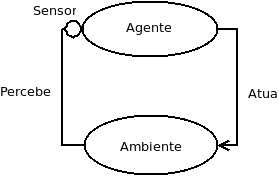
\includegraphics[scale=0.75]{images/agente-basico.png}
	\caption{Esquematização do funcionamento básico de um agente em um ambiente.}
	\label{fig:agente-basico}
\end{figure}

Alguns agentes seguem o princípio de racionalidade básico: sempre objetivam suas ações pela escolha da melhor ação possível segundo seus conhecimentos. Logo é possível inferir que a ação de um agente nem sempre alcança o máximo desempenho, sendo desempenho o parâmetro definido para medir o grau de sucesso da ação de um agente com base nos seus objetivos. São estes os chamados Agentes Racionais.

Como dito anteriormente, agentes estão presentes em um ambiente. O agente não tem controle total do ambiente, ele pode no máximo influenciá-lo com a sua atuação ou criar outros agentes. Podemos separar ambientes em classes: Software, Físico e Relidade virtual (simulação de ambientes reais em software). Em~\cite{wooldridge04} temos, em geral, ambientes com propriedades inerentes à seu funcionamento:

\begin{itemize}
	\item Observável: Neste tipo de ambiente, os sensores dos agentes conseguem ter percepção completa do ambiente. Por exemplo, um sensor de movimento consegue ter visão total em um ambiente aberto.
	\item Determinística: O próximo estado do ambiente é sempre conhecido dado o estado atual do ambiente e as ações dos agentes. O oposto do ambiente determinístico é o estocástico, quando não temos certeza do estado do ambiente. Por exemplo, agentes dependentes de eventos climáticos.
	\item Episódico: A experiência do agente é dividida em episódios, onde cada episódio é a percepção do agente e a sua ação.
	\item Sequêncial: A ação tomada pelo agente pode afetar o estado do ambiente e ocasionar na mudança de estado
	\item Estático: O ambiente não é alterado enquanto um agente escolhe uma ação.
	\item Discreto: Existe um número definido de ações e percepções do agente para o ambiente em cada turno.
	\item Contínuo: As percepções e ações de um agente modificam-se em um espectro contínuo de valores. Por exemplo, temperatura de um sensor muda de forma contínua.
\end{itemize}

Em~\ref{lista_agentes} é mostrado alguns exemplos de agentes, apresentando as suas características já discutidas nesse trabalho.

\begin{table}
	\caption{Listagem de sistemas multiagentes com propriedades de medida de performance, ambiente, atuadores e sensores}
	\begin{tabular}{|p{3cm} | p{3cm} | p{2cm}| p{3cm} | p{3cm} |}
		\hline
		\textbf{Tipo de agente}	& \textbf{Medida de performance} & \textbf{Ambiente} & \textbf{Atuadores}  & \textbf{Sensores}	\\
		\hline
		Sensores de estacionamento	& Avarias no veículo & Carro e garagens & Freio do carro, controle de velocidade & Sensor de proximidade	\\
		\hline
		Jogos com oponente computador	& Quantidade de vitórias &	Software & Realizar jogada & Percepção do tabuleiro	\\
		\hline
		Agentes hospitalares		& Saúde do paciente & Paciente, ambiente médico & Diagnósticos & Entrada de sintomas do paciente	\\
		\hline
	\end{tabular}
	\label{lista_agentes}
\end{table}
 
A primeira linha da tabela~\ref{lista_agentes} apresenta um exemplo de agente atuando em um veículo como um sensor de estacionamento. Responsável por auxiliar o motorista no ato de estacionar o carro, o seu ambiente é da classe físico (considerando o carro e o ambiente onde está o carro). Seu sensor de proximidade é a percepção do ambiente e, caso detecte que está próximo de um obstáculo, pode atuar nos freios dos carros diminuindo a velocidade e evitando colisões. Avarias no carro podem indicar um mal funcionamento do sensor.

A segunda linha da tabela é apresentado o exemplo de agente atuando em um jogo avulso. Esse ambiente é dito dinâmico, pois a cada jogada de um oponente (real ou não), o agente deve analisar a jogada feita pelo seu oponente, irá calcular sua próxima jogada e a realizará. O objetivo principal do agente é a vitória. O ambiente que o agente atua é um software e o seu atuador é um algum mecanismo que permite que ele realize a jogada. O sensor é o mecanismo no qual o agente irá perceber a jogada realizada pelo oponente.

Por fim, a última linha da tabela~\ref{lista_agentes} expõe um exemplo de um agente médico atuando em um ambiente estático: Um paciente. Esse ambiente é classificado como estático por não ser alterado pelo agente nesse exemplo, porém é possível ser diferente em outras situações. O objetivo principal é monitorar a saúde do paciente, logo a medida de performance será a aproximação ou não do diagnóstico médico. Seu atuador não será diretamente no ambiente (corpo humano), será na forma de relatórios médicos e seus sensores podem variar de acordo com a doença a ser monitorada.

Os agentes possuem características inerentes à abordagem~\cite{wooldridge04}. Os agentes possuem os aspectos de~\emph{reatividade},~\emph{proatividade} e~\emph{habilidade social}. O conceito de reatividade  está ligado com o agente perceber o ambiente e reagir. Proatividade é a característica do agente tomar a iniciativa e agir sem a necessidade de nenhum estímulo. Habilidade social é a capacidade de interação com outros agentes.

Os agentes possuem também os seguintes aspectos: Mobilidade, veracidade, benevolência, racionalidade e cooperação. As definições são:
\begin{itemize}
	\item Mobilidade: O Agente deve pode mover-se no ambiente, por exemplo, em uma rede.
	\item Veracidade: Agente não comunica informações falsas.
	\item Benevolência: Agente ajudará os outros.
	\item Racionalidade: O agente não irá agir de forma a impedir a realização de seus objetivos.
	\item Cooperação: O agente coopera com o usuário.
\end{itemize}

\subsection{Arquitetura de agentes}

A arquitetura de agentes varia de acordo com a complexidade da sua autonomia, ou seja, com a capacidade de reagir aos estímulos do ambiente. Conforme verificado em~\cite{novig95}, os tipos de arquitetura são: orientadas à tabela, reflexiva simples, reflexiva baseado em modelo, baseada em objetivo, baseada em utilidade.

A primeira arquitetura a ser explorada é o agente orientado à tabelas. Todas as ações dos agentes dessa arquitetura são conhecidas e estão gravadas em uma tabela. Assim, quando o agente receber o estímulo ele já terá a ação a ser tomada previamente gravada em sua memória. Logo para construir esse tipo de agente, fica claro que além de saber todas percepções possívels, será necessário definir ações apropriadas para todas. Isso levará a tabelas muito complexas e o tamanho pode facilmente passar a ordem de milhões dependendo do número de entradas.

A arquitetura reflexiva simples é um dos tipos mais simples de agente. Nele, o agente seleciona a ação com base unicamente na percepção atual, desconsiderando assim uma grande tabela de decisões. A decisão é tomada com base de regras condição-ação: Se uma condição ocorrer, uma ação será tomada. Por exemplo, vamos supor um agente médico que determina o diagnóstico de uma doença no paciente caso exista alguma anomalia no organismo (Por exemplo, paciente com febre). Uma condição-ação poderia ser:

if anomalia-organismo then diagnóstico-médico

Esse tipo de agente é bastante simples, o que é uma vantagem comparado à arquitetura de tabela. Porém, essa abordagem requer um ambiente totalmente observável, visto que esse tipo de agente possui uma inteligência bastante limitada. No exemplo do agente médico existem diversas maneiras de se detectar uma anomalia no organismo do paciente, seria necessário conhecer todas as formas para usarmos uma abordagem reativa simples.

A arquitetura baseada em modelos funciona de maneira similar a anterior. Nessa abordagem, é levado em conta a parte do ambiente que não é visível neste momento. E para saber o ``momento atual'' de um agente, é necessário guardar a informação de estado consigo. Para atualizar o estado do agente, é necessário conhecer como o mundo desenvolve-se independente do agente (no caso do exemplo, como o organismo funciona) e é necessário saber as ações dos agentes no ambiente. O agente que usa esse tipo de abordagem é chamado de agente baseado em modelo.

Na arquitetura baseada em objetivo, as ações do agente são tomadas apenas se o aproximam de alcançar um objetivo. Para isso, será necessário algo além do estado atual do ambiente: Será necessário informações do objetivo a ser atingido. Assim o agente pode combinar as informações do estado e o objetivo para determinar se deve ou não agir sobre o ambiente. Essa arquitetura porém é obviamente mais complexa e de certa forma ineficiente. Porém ela permite uma maior flexibilização das ações em determinados ambientes, visto que suas decisões são representadas de forma explícita e podem ser modificadas. É interessante notar que esse tipo de arquitetura não trata ações com objetivos conflitantes.

E por fim, a arquitetura baseada em utilidade não utiliza apenas objetivos para realizar a próxima decisão, mas dá ao agente a capacidade de fazer comparações sobre o estado do ambiente e as ações a serem tomadas: Quais delas são mais baratas, confiáveis, resilientes e rápidas do que as outras. A capacidade de avaliação do agente é chamada de função de utilidade, que mapeia uma sequência de estados em um número real que determina o grau de utilidade. Esse mecanismo possibilita a decisão racional de escolha entre vários objetivos conflitantes. Por exemplo, escolher entre um objetivo mais barato ao invés de escolher entre o mais rápido.

\subsection{Sistemas Multiagentes}

Sistemas multiagentes são sistemas compostos por vários agentes capazes de se comunicar, possuindo uma linguagem de alto nível para isso. Um agente possui um objeto que, normalmente, é distinto dos objetivos de outros agentes e pode ou não cooperar com outros agentes para a realização de uma tarefa.

Em~\cite{sarmento11}, podemos encontrar as seguintes características principais em ambientes multiagente:
\begin{itemize}
	\item Fornecem protocolos específicos para comunicação e interação. Cada ambiente tem as suas particularidades: Alguns são em uma única máquina, outros são compartilhados com o mundo real e outros são distribuídos. Cabe a cada ambiente definir um protocolo onde todos agentes devem obedecer para comunicar-se.
	\item São tipicamente abertos.
	\item Contém agentes que são autônomos e individualistas.
\end{itemize}

É trivial imaginar que um sistema multiagente é designado para a solução de problemas de forma distribuída, onde o problema é distribuído entre os agentes que, juntos, trabalham concorrentemente para a resolução deste problema, podendo ou não trabalhar de forma cooperativa.

É importate notar a distinção de conceitos como~\emph{cooperação} na literatura de sistemas multiagentes. Em~\cite{wooldridge04}, existem duas principais diferenças do conceito entre as duas abordagens.

A primeira delas é que agentes são designados de forma diferente, com objetivos diferentes. Em um ambiente com vários agentes, eles devem trabalhar estratégicamente para alcançar seus objetos. A possibilidade de agentes não cooperarem é perfeitamente plausível.

A segunda diferença está no fato do agente agir de forma autônoma, ou seja, tomar suas próprias decisões em tempo de execução sem interferências humanas ou de outros agentes. Logo, um ecossistema de agentes deve ser capaz de coordenar dinâmicamente suas ações, cooperando com outros agentes para atingir os objetivos. Em aplicações distribuídas, esses comportamentos já são desenhados durante o planejamento do software.

A forma de agentes resolverem problemas foi baseada na técnica distribuição cooperativa de resolução de problemas -~\emph{cooperative distributed problem solving} (CDPS). Em~\cite{durfee89}, a técnica CDPS consiste de uma rede de baixo acoplamento provida de sofisticados nós resolvedores de problemas que precisam cooperar entre si, pois nenhum deles possui recursos, informações e~\emph{expertise} suficientes para resolver algum problema sozinho. Cada nó possui uma~\emph{expertise} diferente que pode resolver parte do problema.

Inicialmente essa técnica assumiu que os problemas fossem de ordem benevolente. Isso significa que, implicitamente, os agentes compartilham o mesmo objetivo de resolver o problema proposto. Isso implica que todos os agentes ajudarão sempre que possível, mesmo tendo prejuízos na execução da ação, pois o objetivo geral de todos será a resolução do problema maior. Esse cenário é plausível desde que uma organização ou entidade tenha o controle de (ou modele) todos os agentes.

Em um cenário mais realista (e de maior enfoque dos estudos de SMA), agentes podem pertencer à sociedades com interesses próprios, diferentes de outras sociedades. Logo, é possível ocorrer o conflito de interesses neste ambiente, situação que força os agentes a cooperarem com os outros para alcançarem seus objetivos.

O processo CDPS pode ser divido em três etapas:
\begin{itemize}
	\item decomposição do problema.
	\item solução do subproblema.
	\item integração da solução.
\end{itemize}

Com uma solução compartilhada de resolução de problemas, a arquitetura de sistemas multiagentes mostra-se bastante robusta neste quesito. É necessário porém saber dos detalhes da comunicação entre os agentes, a forma de envio das mensagens, as suas linguagens, bem como outras particularidades.

\subsection{Comunicação}

A comunicação é um dos aspectos mais importantes no desenvolvimento de SMAs. Problemas de sincronização entre as partes que se comunicam devem ser devidamente estudados. A situação mais simples possível da comunicação, onde o agente A envia uma mensagem ao agente B que está prontamente disponível para receber a mensagem nem sempre é a o cenário mais recorrente. Para tanto, é necessário entender os pormenores da comunicação nesta abordagem.

Em uma aplicação normal (Desktop ou Web), a comunicação entre objetos pode ser mais simplificada. Por exemplo, supondo uma aplicação em que existe dois objetos,~\emph{a} e~\emph{b} e que o objeto~\emph{a} tenha um método público chamado~\emph{m1}. O objeto~\emph{b} pode ser comunicar com o objeto~\emph{a} por meio do método~\emph{m1}, provavelmente da seguinte forma~\emph{a.m1(args)}, onde~\emph{args} são os argumentos enviados ao objeto~\emph{a} e a sintaxe pode ser diferente da apresentada, dependendo da linguagem de programação. É importante notar que o controle da execução do método~\emph{m1} não está no objeto~\emph{a}, mas sim no objeto~\emph{b}, que decide o momento o qual o método será invocado.

Esse cenário de comunicação é diferente em um ambiente SMA. Supondo dois agentes~\emph{a} e~\emph{b}, onde o agente~\emph{a} tem a capacidade de executar a ação $\alpha$. O agente~\emph{b} não poderá invocar diretamente o método que corresponde à ação $\alpha$, visto que os agentes são autônomos e independentes: Cada um tem somente tem total controle sobre suas ações e seus estados. O agente precisará enviar a solicitação da execução da ação $\alpha$ por meio de mensagem. Isso porém não garante que o agente~\emph{a} executará esta ação, pois pode não ser do seu interesse. Os agentes podem também influênciar o comportamento de outros agentes, alterando seu estado interno para a execução de ações e cooperando para o cumprimento do objetivo de outros agentes.

A comunicação dos agentes é baseada na teoria dos atos de fala (do inglês~\emph{Speech act theory}) e trata a comunicação como uma ação. A teoria dos atos de fala, publicada em 1962~\cite{austin62} por John Austin, onde ele percebe que certas expressões de linguagem natural, ou atos de fala, possuem a característica de realizar ação em um interlocutor, causando assim uma mudança de de estado da mesma forma que uma ação física. Logo, as expressões descrevem as ações por meio de desejos, habilidades e crenças.

Em~\cite{verschueren09}, a teoria dos atos de fala possuem duas características:
\begin{itemize}
	\item A distinção entre um o significado expressado por uma expressão e a forma como essa expressão é utilizada.
	\item Expressões de todos os tipos podem ser considerados como atos, pois mudam o mundo de alguma forma.
\end{itemize}

Posteriormente o trabalho de John Searle~\cite{searle69}, relacionado ao de Austin, separa uma ação de um ato entre orador(~\emph{speaker}) e ouvinte(~\emph{hearer}) identifinca propriedades e conduções que um discurso deve conter para realizar ações sucedidas. Além disso, ele classifica alguns atos de discursos em 5 classes:
\begin{itemize}
	\item Representativas - Representa o ato de um orador representar uma verdade para o ouvinte. Pode ser entendido como uma ação de informar(\emph{inform}).
	\item Diretivas - Tentativa do orador de fazer algum ouvinte realizar alguma ação por meio do seu ato.. Pode ser entendido como uma ação de requisição(\emph{request}).
	\item Comissivas - O orador toma alguma atitude em relação à uma ação em andamento.
	\item Expressivas - Expressa algum estado psicológico.
	\item Declarações - Causa algum efeito relacionado a determinado assunto.
\end{itemize}

A comunicação então baseia-se nos atos de fala para prever a interação com seres humanos e é definida por meio de semânticas definidas pela teoria da Inteligência Artificial~\cite{wooldridge04}. O formalismo para a comunicação foi escolhido de forma que foi possível representar os atos de discursos em uma lógica multimodal, que contém os operadores de desejos, habilidades e crenças dos atos de discurso.

Da mesma forma que a teoria dos atos de fala influênciou na arquitetura da comunicação, ela influênciou também nas várias linguagens de comunicação dos agentes. Linguagens foram desenvolvidas para, não apenas representar ações de agentes, mas também para representar o conhecimento entre sistemas autônomos. No início dos anos 90, duas linguagens foram desenvolvidas pelo consórcio~\emph{Knowledge Sharing Effort}, encabeçados pela agência norte americana~\emph{Defense Advanced Research Projects Agency}(DARPA)~\cite{kse}.
\begin{itemize}
	\item ~\emph{Knowledge Query and Manipulation Language} (KQML) - Protocolo designado para a comunicação de agentes, em uma arquitetura que esses agentes sejam projetados para resolver problemas da arquitetura cliente-servidor~\cite{preece1997}. Não existe o foco com o conteúdo da mensagem.
	\item \emph{Knowledge Interchange Format} (KIF) - Criada para facilitar a troca de conhecimento entre agentes, suas declarações são providas de significados que podem ser compreensíveis a qualquer agente que conheça a estrutura da linguagem. Não possui foco na transmissão da mensagem~\cite{kifmanual}.
\end{itemize}

\subsubsection{KQML}

A linguagem KQML define um protocolo para comunicação de agentes, onde cada mensagem tem um enunciado performativo (~\emph{performative}), que varia com o seu objetivo, e em seguida os parâmetros da mensagem. O KQML define vários enunciados performativos que distinguem-se pelo objetivo da mensagem, sendo dividas em três categorias: Discursivas, intervenção/mecânica e facilitação e~\emph{networking}. Por exemplo, uma mensagem com o tipo performativo~\emph{ask-one} indica que o agente remetente A deseja saber uma resposta do agente B sobre o conteúdo da mensagem. Em~\cite{preece1997}, é possível verificar que a última versão da linguagem define mais de trinta enunciados performativos.

Os maioria dos parâmetros são opcionais, sendo os mais importantes: \emph{content} e ~\emph{receiver}. A tabela~\ref{parametros_kqml} lista os principais parâmetros em uma mensagem nesta linguagem, bem como seu significado.

\begin{table}
	\caption{Listagem de atributos de uma mensagem em KQML}
	\begin{tabular}{|p{3cm} | p{12cm} |}
		\hline
		\textbf{Parâmetro}	& \textbf{Significado}	\\
		\hline
		\emph{sender}		& Remetente da mensagem. \\
		\hline
		\emph{receiver}	& Destinatário da mensagem. \\
		\hline
		\emph{reply-with}	& Identifica se o remetente espera uma respota. Em caso positivo, o campo~\emph{in-reply-to} deve ser preenchido com a referência para a resposta. \\
		\hline
		\emph{in-reply-to}	& Campo conténdo a referência para a resposta solicitada. \\
		\hline
		\emph{language}	& Linguagem em que o campo~\emph{content} está escrito. \\ 
		\hline
		\emph{ontology}	& Indica a forma que deve ser interpretada o conteúdo do campo~\emph{content}. \\
		\hline
		\emph{content}		& Conteúdo da mensagem. \\
		\hline
	\end{tabular}
	\label{parametros_kqml}
\end{table}
O formato da mensagem é completamente compreensível aos humanos. Na mensagem~\ref{code:exemplo-kqml} podemos verificar na primeira linha o enunciado performativo~\emph{ask-one}, onde será uma mensagem de consulta. Nas linhas abaixo, visualizamos todos os parâmetros da mensagem antecedidos por (:). O primeiro parâmetro da mensagem é~\emph{receiver} como controle-estoque, ou seja, esse será o destinatário da mensagem. O segundo parâmetro~\emph{language} tem o valor PROLOG indicando que a sintaxe do conteúdo está escrita em PROLOG. O próximo parâmetro,~\emph{ontology} informa a ontologia que espressa o conteúdo. Por fim, o parâmetro~\emph{content} que indica o conteúdo da mensagem, no caso, uma consulta escrita em PROLOG perguntando pelo preço de um computador.

\begin{lstlisting}[label=code:exemplo-kqml,caption=Exemplo de mensagem em KQML]
(ask-one
	:receiver controle-estoque
	:language PROLOG
	:ontology PRODUTOS
	:content  (PRECO COMPUTADOR ?price)
)
\end{lstlisting}

Um exemplo de diálogo escrito em KQML pode ser visto na sequência de mensagens~\ref{code:dialogo-kqml}

\begin{lstlisting}[label=code:dialogo-kqml,caption=Exemplo de diálogo em KQML]
(evaluate
	:sender A
	:receiver B
	:language PROLOG
	:ontology PRODUTOS
	:reply-with q1
	:content  (PRECO COMPUTADOR ?price)
)
(reply
	:sender B
	:receiver A
	:language PROLOG
	:ontology PRODUTOS
	:in-reply-to q1
	:content  (=2000.00)
)
\end{lstlisting}

A primeira mensagem do diálogo possui o enunciado performativo é~\emph{evaluate}, significando que o emissor A deseja avaliar o conteúdo com B. Nos parâmetros é possível notar que a linguagem da mensagem é PROLOG, utiliza a ontologia PRODUTOS e o conteúdo é uma consulta em prolog. O parâmetro~\emph{reply-with} cria uma referência para a consulta do conteúdo conteúdo.

Na segunda mensagem, o seu enunciado performativo é~\emph{reply}, significando uma mensagem do tipo resposta. O parâmetro~\emph{in-reply-to q1} especifica essa mensagem como resposta à q1, ou seja, à consulta da mensagem anterior. Dessa forma a linguagem consegue distinguir respostas de um mesmo remetente. Os outros parâmetros são o emissor B, destinatário A, linguagem PROLOG e o conteúdo da mensagem, o valor da consulta q1.

Em~\cite{wooldridge04}, a adoção desta linguagem pela comunidade de SMA foi significante, mas sofreu diversas críticas:
\begin{itemize}
	\item A fluídez e a não restrição do KQML fez com que diversas implementações extendidas surgissem, impossibilitando a interoperabilidade entre sistemas.
	\item Mecanismos de transporte do KQML nunca foram bem definidos, causando problemas de diversas implementações destes mecanismos e prejudicando novamente a interoperabilidade.
	\item A semântica do KQML nunca foi formalmente definida, ocasionando em má interpretações dos enunciados performativos.
	\item A linguagem não possui enunciados performativos adequados para algumas semânticas. Por exemplo, a inexistência do enunciado~\emph{comissives}.
\end{itemize}

Dessa forma, novos desenvolvimentos de linguagens fizeram-se necessários.

\subsubsection{KIF}
A linguagem foi desenvolvida para expressar conhecimento a cerca de um determinado domínio, sendo possível assim a troca de conhecimentos entre agentes. Em~\cite{kifmanual}, a linguagem possui as seguintes características:
\begin{itemize}
	\item Tem uma semântica declarativa, sendo possível entender o seu significado sem a necessidade de um interpretador para manipulação das expressões.
	\item É logicamente compreensível.
	\item É provida com a capacidade de reproduzir meta-conhecimento, ou seja, conhecimento a respeito da representação do conhecimento. Com isso, é possível reproduzir novas representações de conhecimento sem a necessidade de modificar a linguagem.
\end{itemize}

A linguagem é baseada na lógica de primeira ordem onde são definidos operadores como existe($\exists$) e para todo($\forall$),possibilitando aos agentes a expressão de diversas propriedades, domínios, dentre outros. Além disso, ela define um vocabulário básico para a expressão de tipos básicos (números, caracteres, strings) e algumas funções padrões para lidar com esses tipos de dados (menor que, maior que, soma, dentre outros). 

O trecho de código~\ref{code:exemplo-kif} ilustra um exemplo de expressão na linguagem KIF, validando que a temperatura de m1 é 83 graus Célsius.

\begin{lstlisting}[label=code:exemplo-kif,caption=Exemplo de expressão de conteúdo com a linguagem KIF. Fonte:~\cite{wooldridge04}]
(= (temperature ml ) ( scalar 83 Celsius))
\end{lstlisting}

\subsection{Linguagem de Comunicação de Agentes FIPA}

Após as críticas à linguagem KQML, o consórcio~\emph{Foundation for Intelligent Physical Agents} (FIPA) começou a trabalhar em 1995 no desenvolvimento da padronização de SMAs. O núcleo dessa padronização foi o desenvolvimento de uma linguagem de comunicação de agentes (ACL) padronizada para todas as plataformas.

Baseado na linguagem KQML, a estrutura das mensagens é a mesma e os seus atributos são semelhantes. A maior diferença entre as duas linguagens são os enunciados performativos. Foram definidos 20 tipos de mensagens performativas, muito semelhante ao KQML, porém definindo formalmente as interpretações dessas mensagens e não definindo nenhuma linguagem para o conteúdo da mensagem.

Devido ao fato da linguagem KQML não ter performativos adequados, a ACL da FIPA recebeu total preocupação na definição formal da semântica da linguagem. A tabela~\ref{table:fipa-cal-spec} contém um breve resumo dos enunciados performativos disponíveis em~\cite{fipa-cal-spec}. É importante notar que a especificação~\cite{fipa-cal-spec} possui toda a descrição formal de cada enunciado performativo aqui descrito.

\begin{table}
	\caption{Listagem de Enunciados Performativos}
	\begin{tabular}{|p{3cm} | p{12cm} |}
		\hline
		\textbf{Tipo}	& \textbf{Descrição}	\\
		\hline
		\emph{Accept Proposal} & Declaração de aceite de proposta feita por um agente.	\\
		\hline
		\emph{Agree} & Performativa feita por um agente indicando que aceitou o~\emph{request} feito por outro agente.	\\
		\hline
		\emph{Cancel} &	Cancela uma mensagem de~\emph{request}, informando que não irá mais participar daquela conversação.  \\
		\hline
		\emph{Call for Proposal} & Performativo que indica o início de uma negociação entre agentes.	\\
		\hline
		\emph{Confirm} & A confirmação permite ao emissor da mensagem confirmar a veracidade do conteúdo da mensagem.	\\
		\hline
		\emph{Disconfirm} & Similar à confirmação, porém informando ao emissor da não certeza do conteúdo da mensagem.	\\
		\hline
		\emph{Failure} & Permite ao agente indicar que a tentativa de executar uma ação falhou.	\\
		\hline
		\emph{Inform} & Informa à um destinatário que o conteúdo da mensagem é verdadeiro, implicando que o remetente da mensagem também acredita no seu conteúdo. É uma das mais importantes performativas feitas pela FIPA.	\\
		\hline
		\emph{Inform If} & Envia uma mensagem a qual o seu conteúdo pode ser verdadeiro ou falso.	\\
		\hline
		\emph{Inform Ref} & Similar ao \emph{Inform If}, com a diferença que ao invés de questionar se é verdadeiro ou falso, ele solicita o valor de uma expressão para o remetente.	\\
		\hline
		\emph{Not Understood} & Informa à um agente que não entendeu por que determinada ação deve ser realizada. Usada quando o estado interno do agente não é compatível com a mensagem.	\\
		\hline
		\emph{Propagate} & Consiste em propagar o conteúdo da mensagem para um grupo de agentes.	\\
		\hline
		\emph{Propose} & Permite um agente realizar uma proposta em uma negociação para outro agente.	\\
		\hline
		\emph{Proxy} & Permite ao destinatário da mensagem agir como um~\emph{proxy} para os agentes que estão descritos no conteúdo da mensagem.	\\
		\hline
		\emph{Query If} & Permite à um agente consultar um destinatário sobre a validade do conteúdo.	\\
		\hline
		\emph{Query Ref} & Similar ao \emph{query-if}, porém o agente remetente irá consultar o valor de uma expressão	\\
		\hline
		\emph{Refuse} & Indica que um determinado agente não irá executar uma ação que foi determinada por outro agente.	\\
		\hline
		\emph{Reject Proposal} & Permite um agente rejeitar uma proposta feita por outro agente em uma negociação.	\\
		\hline
		\emph{Request} & Permite à um agente requisitar que outro agente execute determinada ação.	\\
		\hline
		\emph{Request When} & Permite à um agente requisitar que outro agente execute determinada ação quando a proposição (no conteúdo da mensagem) for verdadeira.	\\
		\hline
		\emph{Request Whenever} & Similar ao \emph{request-when}, porém o agente nunca irá executar a ação quando a proposição (no conteúdo da mensagem) for verdadeira.	\\
		\hline
		\emph{Subscribe} & O conteúdo será uma proposição e o remetente da mensagem será notificado sempre que essa proposição for verdadeira.	\\
		\hline
	\end{tabular}
	\label{table:fipa-cal-spec}
\end{table}

As performativas~\emph{request} e~\emph{inform} consideradas principais pela especificação da FIPA, pois orientam toda a linguagem de comunicação. Além disso, é possível derivar as outras performativas por meio delas.


\subsection{Ontologias}

Ontologia é um ramo da Filosofia que dedica-se a estudar e representar a natureza do ser, existência ou realidade. É uma formalização dos conceitos e relacionamentos que podem existir em um determinado universo. Para a Inteligência Artificial, é tudo aquilo que pode ser representado. Em o autor~\cite{novig95}, a representação de conceitos e objetos pode ser entendida como Engenharia Ontológica:

\begin{quote}
\emph{...concentrating on general concepts-such as Actions, Time, Physical Objects, and Beliefs - that occur in many different domains. Representing these abstract concepts is sometimes called ontological engineering.}
\end{quote}

A possibilidade de representação de conhecimento por meio de ontologias é bastante vasta. A sua forma de especificação pode ser entendida como uma hierarquia, onde os conhecimentos são organizados na forma de árvore, possibilitando a inserção de novos conhecimento a qualquer momento.

\begin{figure}
	\centering
	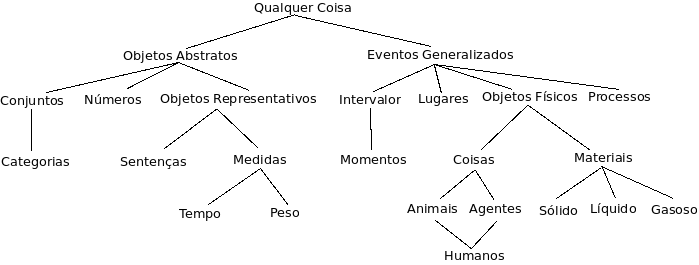
\includegraphics[scale=0.65]{images/arvore-ontologia.png}
	\caption{Ontologias superiores do mundo, cada uma indicando um conceito ou especialização do seu superior.}
	\label{fig:arvore-ontologia}
\end{figure}

Em~\ref{fig:arvore-ontologia}, é possível observar a organização geral de conceitos, chamado de ontologias superiores. As ontologias gerais estão representadas no topo da árvore, e as suas especialidades vão crescendo no sentido das folhas.

Em um ambiente de Sistemas Multiagentes, além de especificar uma linguagem para comunicação, dois agentes podem comunicar-se com relação à um determinado domínio de aplicação: Podem negociar valores de carteiras em uma organização financeira, podem trocar mensagens sobre os dados analisados de performance de veículos, dentre outros exemplos. Em outras palavras, dois agentes podem comunicar-se usando a mesma ontologia.

Existem muitas linguagens que foram desenvolvidas para expressar ontologias. A mais comum delas é a~\emph{eXtensible Markup Language} (XML), uma linguagem de marcação que organiza os dados de forma hierarquizada.

O exemplo~\ref{code:exemplo-xml} está descrito escrito na linguagem XML que representa o domínio de países. Nele podemos ver a ontologia superior, País. Cada país é composto por um conjunto de estados, conténdo as propriedades nome e sigla. Cada estado possui um conjunto de cidades. Cada cidade possui os atributos nome e população. Esses atributos poderiam ser escritos de forma diferente no trecho~\ref{code:exemplo-xml}, porém sem alteração de semântica.


\begin{lstlisting}[language=xml,label=code:exemplo-xml,caption=Exemplo de código XML representando uma ontologia simples de cidades.]
	<Pais nome="Brasil">
		<Estado nome="Goias" sigla="GO">
			<Cidade>
				<Nome>Goiania</Nome>
				<Populacao>1.300.000</Populacao>
			</Cidade>
			<Cidade>
				<Nome>Anapolis</Nome>
				<Populacao>342.347</Populacao>
			</Cidade>
			<Cidade>
				<Nome>Aparecida de Goiania</Nome>
				<Populacao>474.219</Populacao>
			</Cidade>
		</Estado>
		<Estado nome="Sao Paulo" sigla="SP" >
			<Cidade>
				...
			</Cidade>
			...
		</Estado>
		...
	<Pais>
\end{lstlisting}

\section{Multiagent Systems Engineering}\label{section:mase}

Atualmente muitas abordagens de projeto de desenvolvimento de software conseguem com sucesso definir uma metodologia para construção, implantação e manutenção do software. A definição dessas engenharias de software possuem diversos casos de sucesso em sua maioria nas áreas de Análise de Projetos Orientados à Objetos. O advento de sistemas multiagentes trouxe à tona a necessidade de outras metodologias de desenvolvimento diferente daquelas, devido à diferença de abordagem do software.

Pela característica autônoma dos agentes, não é possível compará-los à simples objetos que serão invocados por outros objetos. Não existe interação direta, apenas coordenação de ações via conversação para cada agente atingir suas próprias métas.

O desenvolvimento de uma metodologia para projetar sistemas multiagentes surgiu, chamada~\emph{Multiagent Systems Engineering} (MASE), onde os requisitos e metas do SMA são levantados e a partir de então as tarefas e agentes são projetadas para lhes atender. O MASE utiliza-se de alguns modelos gráficos para a descrição dos agentes, seus objetivos, suas interações e a sua arquitetura.

Em~\cite{scott01}, a metodologia do MASE é baseada nas mais tradicionais metodologias de desenvolvimento de software, dividida em duas fases principais: Análise e Design.

A primeira fase, chamada de análise, consiste no levantamento e entendimento dos requisitos com o objetivo de um conjunto de regras, as quais são associadas à tarefas que devem ser realizadas para o sistema atingir seus objetivos. No fim dessa fase, alguns artefatos são gerados que nortearão a próxima etapa da metodologia. A fase de análise pode ser dividida nos seguintes três passos:

\begin{itemize}
	\item Capturar Metas
	\item Desenvolver Casos de Uso
	\item Refinar Regras
\end{itemize}

A fase de design consiste na modelagem do SMA de acordo com as regras levantadas na fase anterior. O objetivo é a definição das conversações que existirão entre os agentes, bem como a arquitetura geral do sistema. Essa fase pode ser divida em quatro passos:

\begin{itemize}
	\item Criar as Classes dos Agentes
	\item Construir Conversações
	\item Montagem dos Agentes
	\item Design do Sistema
\end{itemize}

Existem outras metodologias para desenvolvimento de Sistemas Multiagente. A metodologia~\emph{Gaia}~\cite{wooldridge2000} consiste em uma abordagem não iterativa que define análise e~\emph{design} de sistemas baseados em agentes. Esta metodologia é considerada genérica e compreensível pois pode ser aplicada a um nível muito amplo de sistemas multiagente e ela lida tanto com escopos mais gerais (sociedade), quanto com escopos mais específicos (agentes). Ela define as regras e tarefas em termos de uma organização, que é sinônimo de sociedade de agentes ou sistemas multiagentes.

A metodologia~\emph{PASSI} (\emph{Process for Agent Societies Specification and Implementation}) é designada para o acompanhamento do desenvolvimento do sistema desde o levantamento dos requisitos até a codificação~\cite{burrafato02}. Seus modelos de projetos são baseados nas especificações da FIPA, garantindo assim a compatibilidade com o SMA a ser desenvolvido. O~\emph{PASSI} define uma metodologia cinco modelos de trabalho: Requisito do Sistema, sociedade de Agentes, implementação dos agentes, modelo de código e modelo de implantação.

\subsection{Análise}

Em~\cite{scott01}, a fase de análise objetiva o desenvolvimento de um conjunto de regras, que descrevem uma funcionalidade para uma entidade, as quais as atividades descrevem o que deve ser feito para o sistema atingir o seus objetivos.

\subsubsection{Captura de Metas}

O primeiro passo dessa fase, Captura de Metas, consiste na transformação da especificação inicial do sistema em um conjunto estruturado de metas. Entende-se que as~\emph{metas} que o sistema leva em consideração são relacionadas ao sistema (e não ao usuário), visto que são mais estáveis e as metas do sistema devem satisfazer, de forma geral, os objetivos do usuário~\cite{scott01}.

Dividida em dois subpassos, o primeiro deles é a identificação de todas as metas. A partir da documentação inicial do sistema, conténdo os requisito  funcionais, são extraídos os objetivos de cada cenários do sistema. É importante ressaltar que as metas devem descrer de forma geral e sucinta o comportamento do sistema, descrevendo o que ele deve fazer e não como deve ser feito.

As metas podem ser divididas em 4 tipos, podendo ser classificadas em mais de um: Sumário, particionada, combinada e não funcional. A meta sumário é derivada de outras metas semelhantes para que se generalize em uma meta pai. Meta particionada é a meta que, quando todas suas submetas são atingidas,  a meta passa a ser atingida. Metas combinadas são metas que são agrupadas devido à semelhaça de seus objetivos. As metas não funcionais são relativas à cumprir objetivos que são requisitos não funcionais do sistema.

O segundo subpasso consiste na estruturação de metas em forma hierarquizada. É necessário separar quais metas são mais abstratas e de que forma elas podem ser agrupadas em forma de hierarquia. Com isso, eliminam-se algumas metas que são repetidas e identificam-se quais metas são atingidas por meio de outras submetas.

\subsubsection{Desenvolver Casos de Uso}

Neste passo o objetivo é entender o comportamento e o fluxo de execução do sistema por meio dos casos de uso, além de haver um entendimento maior sobre como o sistema irá se comunicar. Para tanto, este passo visa o levantamento e criação dos casos de uso do sistema, bem como o diagrama de sequência para detalhar a ordem dos eventos de cada cenário.

Os casos de uso geralmente são levantados a partir dos requisitos iniciais do sistema. Nele, são identificados os participantes (atores) e a sua interação com o sistema, esclarecendo a comunicação de alguns módulos do sistema.

O diagrama de sequência define os eventos que cada interação pode criar, mostrando a ordem de execução destes eventos e a sua comunicação. Esses diagramas são criados para cada caso de uso, podendo haver mais de um para cada caso de uso. O objetivo principal é o levantamento dos eventos e das regras.

\subsubsection{Refinar Regras}

O último passo da fase de análise, o refinamento de regas consiste na associação metas e seus diagramas de sequências às regras e suas respectivas tarefas. A associação de tarefas à regras é a melhor forma de modelagem de Sistemas Multiagentes~\cite{scott01}. 

Em geral, a associação de metas às regras é de um para um, não sendo uma regra necessáriamente. Durante esta etapa, algumas considerações relativas ao desenho do sistema devem ser levadas em consideração. Caso exista alguma alteração (adição de uma nova meta, alteração de caso de uso, dentre outras), a metodologia permite que o analista retorne aos passos anteriores e remodele a solução. Algumas metas podem ser combinadas em apenas uma regra, simplificando o desenho do sistema.

A interface com sistemas externos geralmente é tratada como uma regra diferente, visto que sua complexidade pode variar. O MASE não modela explicitamente um ator humano, pois o considera como um ator externo ao sistema.

Após a associação das regras, elas são estruturas em uma modelagem chamada~\emph{MASE Role Model}, conténdo informações de interações entre as tarefas. A representação a notação do~\emph{MASE Role Model}~\ref{fig:exemplo-mase-role-model} utilizada por~\cite{scott01} utiliza-se de retângulos para expressar as regras, elipses para identificar as tarefas e as setas entre as tarefas representam as suas comunicações. Essas comunicações podem ser por meio de mensagens, caso as regras estejam separadas em agentes diferentes.

\begin{figure}
	\centering
	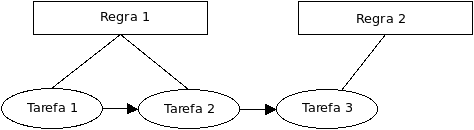
\includegraphics[scale=0.65]{images/exemplo-mase-role-model.png}
	\caption{Representação utilizada no MASE Role Model.}
	\label{fig:exemplo-mase-role-model}
\end{figure}

Caso as regras compartilhem tarefas será necessário remodelar a composição da regra, visto que o MASE não permite a duplicação de tarefas. 

De forma geral, cada regra possui uma série de tarefas que podem (ou não) executar paralelamente. Cada tarefa possui um comportamento que pode depender de outras regras para o cumprimento de seu objetivo. Preocupando-se com as conversações entre tarefas, o MASE determina neste passo a criação do~\emph{Concurrent Task Diagram}.

O diagrama é representado por meio de autômatos de estados finitos~\ref{fig:examplo-diagrama-tarefas-concorrentes}, devido a facilidade de construção e entendimento. A transição consiste de uma mudança de estado do agente, podendo envolver um processamento ou uma comunicação externa.
\begin{figure}
	\centering
	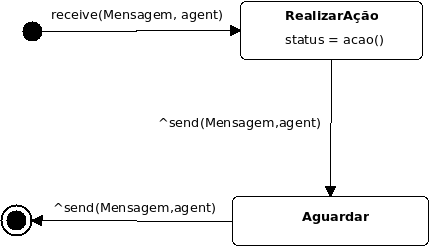
\includegraphics[scale=0.65]{images/examplo-diagrama-tarefas-concorrentes.png}
	\caption{Representação utilizada no~\emph{Concurrent Task Diagram}.}
	\label{fig:examplo-diagrama-tarefas-concorrentes}
\end{figure}

A mudança de estado do automato é equivalente à mudança de estado do agente. A sintaxe da transição de pode ser expressa por meio de uma notação~\ref{code:sintaxe-concurrent-task} que define o gatilho a ser disparado, condições para a execução e as mensagens transmitidas.

\begin{lstlisting}[label=code:sintaxe-concurrent-task,caption=Sintaxe da mudança de estado.]
	trigger [guard] ^ transmission(s)
\end{lstlisting}

O~\emph{token} trigger representa um evento que inicia a mudança de estado, geralmente vindo de outra tarefa da mesma regra. O~\emph{token [guard]} é a verificação da validade do código~\emph{guard}, ocorrendo a mudança de estado somente quando a condição for verdadeira. Por fim ocorrem as transmissões, que podem conter o parâmetro~\emph{s}.

Para comunicações externas, dois eventos especiais foram definidos: O evento~\emph{send} indicando o envio de mensagem e o evento~\emph{receive}, indicando o recebimento de mensagem.

A mensagem sempre possui um cabeçalho performativo (definida pela FIPA, representa o objetivo da mensagem) com a seguinte sintaxe:\emph{performative(p1...pn)}, onde~\emph{p1...pn} indicam os parâmetros da mensagem.

Após a definição dos~\emph{Concurrent Tasks Diagrams}, o analista pode combinar tarefas, a fim de diminuir a complexidade do sistema. 

Com isso, o sistema já possui a complexidade das regras determinadas, bem como as tarefas necessárias para atingir seus objetivos.

\subsection{Design}

A fase de design é divida em quatro passos: Criar Classes dos Agentes, Construir Conversações, Montagem dos Agentes e Design do Sistema. O principal objetivo desta fase é projetar os agentes e suas interações de acordo com os insumos construídos na fase anterior.

\subsubsection{Criando as Classes dos Agentes}

Neste passo, os agentes são criados com base nas regras definidas na fase anterior. Para cada agente criado deve existir pelo menos uma regra associada, caso contrário o levantamento de regras mostra-se incompleto. Dessa forma, o MASE garante que todas os objetivos  do sistema são atingidos, já que as regras do sistema estão relacionados com as metas que foram levantadas na etapa anterior.

Ao fim deste passo é necessário a criação de um novo diagrama, o~\emph{Agent Class Diagram}~\ref{fig:exemplo-agent-class-diagram}. Nele, as classes dos agentes são associadas com as regras levantadas e as comunicações entre as classes.

\begin{figure}
	\centering
	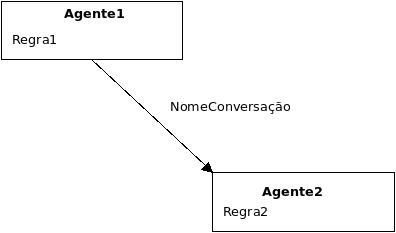
\includegraphics[scale=0.65]{images/exemplo-agent-class-diagram.png}
	\caption{Representação utilizada no~\emph{Agent Class Diagram}.}
	\label{fig:exemplo-agent-class-diagram}
\end{figure}

\subsubsection{Construir Conversações}

A próxima etapa da segunda fase diz respeito às conversações que existirão no SMA. Aqui, cada detalhe da conversação entre dois agentes deverá ser planejado para que haja a correta comunicação entre os agentes e a quantidade de erros seja minimizada.

Quando o agente recebe uma mensagem, ele automaticamente compara com as suas conversações ativas~\cite{scott01}. Caso exista alguma conversação semelhante, o agente muda o seu estado e realiza as ações relativas para atingir esse estado. Caso contrário, é assumido que o agente emissor deseja iniciar uma nova conversação e o receptor compara com as suas possibidades de tipos de conversação disponíveis para participar.

Neste passo, é criado o Diagrama de Comunicação. Nele, as conversações são montadas por meio do mesmo autômato de estados finitos, utilizado na fase análise, passo~\emph{refinar regras}. Os estados do aumtômato são as ações que devem ser realizadas pelo agente. As transições de estado são as conversações que são feitas pelo agente.

A sintaxe usada na conversação de agentes~\ref{code:sintaxe-conversation} é uma expressão que é definida por meio das mensagens recebidas, condições, ações e mensagens transmitidas. O~\emph{token rec-mess} indica que a mensagem com os parâmetros~\emph{args1} foi recebida caso a condição~\emph{cond} seja verdadeira. Então o método~\emph{action} é chamado e a mensagem~\emph{trans-mess} com os argumentos~\emph{args2}. Todos os elementos da mensagem são opcionais.

\begin{lstlisting}[label=code:sintaxe-conversation,caption=Sintaxe da conversação entre dois agentes.]
	rec-mess(args1) [cond] / action ^ trans-mess(args2)
\end{lstlisting}

O Diagrama de Comunicação~\ref{fig:exemplo-conversation} é definido para os dois lados da conversação: Iniciador e Receptor. considerando o lado iniciador da conversação.

\begin{figure}
	\centering
	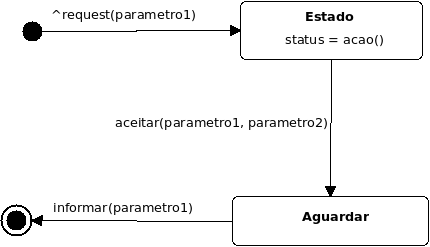
\includegraphics[scale=0.65]{images/exemplo-conversation.png}
	\caption{Exemplo de conversação utilizada no Diagrama de Comunicação do lado do iniciador da conversação.}
	\label{fig:exemplo-conversation}
\end{figure}

\subsubsection{Montagem dos Agentes}

Neste passo, o estado interno dos agentes é criado. É necessário nesta etapa definir a arquitetura dos agentes e os componentes que irão compor esta arquitetura. Para isso, é necessário criar o Diagrama de Arquitetura de Agentes, onde são representados os componentes arquiteturais dos agentes.

Os componentes internos dos agentes podem ser atributos dos agentes, ou métodos auxiliares. Um agente pode ter vários componentes internos e estes componentes obviamente se comunicarão. No mínimo, cada agente criado no Diagrama de Agentes deve ser definir uma arquitetura interna.

No Diagrama de Arquitetura de Agentes~\ref{fig:exemplo-diagrama-arquitetura-agentes}, a linha tracejada significa interação com sistemas externos, enquanto a outra significa interação com outros agentes do sistema.

\begin{figure}
	\centering
	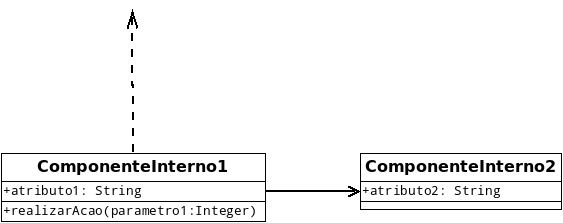
\includegraphics[scale=0.65]{images/exemplo-diagrama-arquitetura-agentes.png}
	\caption{Notação utilizada na arquitetura de agentes.}
	\label{fig:exemplo-diagrama-arquitetura-agentes}
\end{figure}

As setas tracejadas indicam dependência com atributos externos ao agente, enquanto as outras setas representam dependência entre componentes.

\subsubsection{Design do Sistema}

A fase final da metodologia MASE consiste na criação de um diagrama de~\emph{deploy} dos agentes. Este diagrama consiste na representação do número de agentes que serão criados por cada máquina da aplicação, bem como suas localizações no sistema.

A representação do diagrama de~\emph{deploy}~\ref{fig:exemplo-diagrama-deploy} expressa os ambientes criados, bem como os agentes internos. O retângulo com linhas pontilhadas representam os ambientes que podem existir na aplicação. Os outros retângulos caixas representam os agentes e as linhas que os ligam representam as suas interações.

\begin{figure}
	\centering
	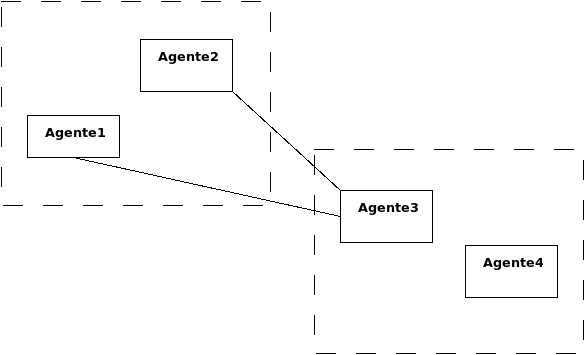
\includegraphics[scale=0.65]{images/exemplo-diagrama-deploy.png}
	\caption{Notação utilizada no diagrama de deploy.}
	\label{fig:exemplo-diagrama-deploy}
\end{figure}

\subsubsection{Ferramenta~\emph{AgentTool}}

O~\emph{AgentTool} é uma ferramenta que dá suporte à metodologia MASE para desenvolvimento de Sistema Multiagente. A versão 1.8.1 dá suporte à todas fases e passos do MASE~\cite{agentTool2012}, provendo suporte para a criação de diagramas, detalhamento de conversações e casos de uso simplificados.



\section{Ferramentas Utilizadas}

Nesta seção estão reunidos as tecnologias que auxiliares ao desenvolvimento do SMA. A primeira seção explica alguns diagramas que são definidos na~\emph{Unified Modeling Language}, necessários para entender os passos da~\emph{Multiagent System Engineering}.
 
Em seguida é explicado os conceitos relacionados ao~\emph{middleware} JADE, bem como a sua arquitetura, o funcionamento dos agentes e os agentes que possuem interface gráfica.

Por fim, este capítulo disserta a respeito da ferramenta JBoss Seam, responsável por interligar os principais~\emph{frameworks} JAVA e facilitar o desenvolvimento de aplicações Web dinâmicas.

\subsection{Unified Modeling Language}

A Linguagem Unificada de Modelagem,~\emph{Unified Modeling Language} (UML) é uma linguagem visual que foi desenvolvida para a representação do software por meio de imagens, objetivando o entendimento dos artefatos de forma rápida e clara e resultando em uma semântica para o projeto em questão. Em~\cite{fowler04} o UML faz parte de uma família de notações gráficas que ajudam na descrição e concepção de sistemas de software, principalmente em sistemas concebidos utilizando o paradigma da orientação à objetos (OO).

O UML é um padrão não proprietário, controlado pelo consórcio~\emph{Object Management Group}~\cite{omg20}. Seu nascimento é datado em 1997~\cite{fowler04}, surgindo a partir da união de diversas linguagens e ferramentas de surgiram na década de 80 e 90.
A linguagem ajuda o entendimento de como o software foi projetado, como ocorre a comunicação entre seus objetos, como suas classes são organizadas, quais são os atores que são envolvidos na utilização do software, dentre outras possibilidades de representação.

É possível separar o uso do UML de três formas distintas~\cite{fowler04}, diferindo entre as modelagens utilizadas e o objetivo de uso. As três formas são: Rascunho, planta de software e como linguagem de programação. 

A utilização como rascunho é utilizada para facilitar a comunicação entre as pessoas envolvidas no projeto, sejam desenvolvedores discutindo funcionalidades do software ou gestores explicando funcionalidades em alto nível. O objetivo neste uso é a comunicação de alguns aspectos do sistema de forma rápida, sem a necessidade de formalizar artefatos para o projeto.

A utilização do UML como planta de software são documentos detalhados que são criados para documentação do software, sendo divida em duas sub-categorias: Engenharia reversa e engenharia normal. Na engenharia reversa, os diagramas são gerados a partir de uma ferramenta que faz a leitura do código fonte e gera os diagramas desejados, que são utilizados para auxiliar o leitor no entendimento do sistema. Na engenharia normal, a idéia é modelar o sistema detalhadamente antes de qualquer desenvolvimento, prevendo quais serão os módulos do sistema, bem como a sua a comunicação.

No uso como linguagem de programação, o UML é utilizado para geração de código executável por ferramentas avançadas de modelagem. Esse modo requer a modelagem de estado e comportamento do sistema, para fins de detalhar todo o comportamento e lógica do sistema em código.

\subsubsection{Diagramas UML}

O UML 2.0 descreve 13 tipos de diagramas~\ref{fig:categorias-diagramas} que podem ser categorizados como estruturais e comportamentais

\begin{figure}
	\centering
	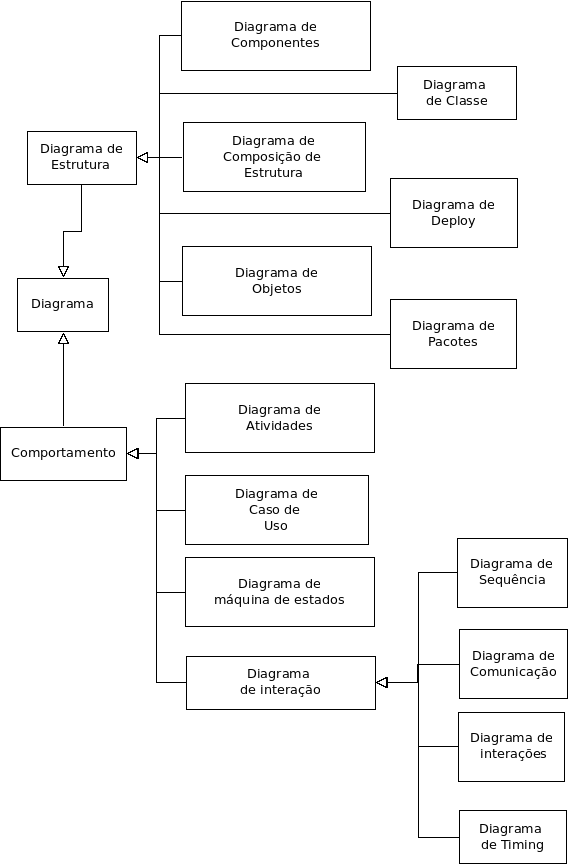
\includegraphics[scale=0.75]{images/categorias-diagramas.png}
	\caption{Categorização dos Diagramas UML 2.0. Adaptado de~\cite{fowler04}.}
	\label{fig:categorias-diagramas}
\end{figure}

Apesar da grande quantidade diagramas envolvidos no UML, nem todos os processos de desenvolvimentos de software utilizam todos eles. Em~\cite{larman08}, a grande extensão de diagramas UML não é usada pela maioria das metodologias. A metodologia de desenvolvimento de sistema multiagente utiliza-se apenas dos seguintes diagramas:

\begin{itemize}
	\item Diagrama de Caso de uso
	\item Diagrama de Sequência
\end{itemize}

\paragraph{Diagrama de Caso de Uso}
Casos de uso são relatos textuais que são utilizados para descobrir e descrever os requisitos do sistema. Consiste da descrição de como um ator utiliza uma funcionalidade do sistema para atingir algum objetivo relacionado. Em~\cite{larman08}, os casos de uso devem ser prioritariamente desenvolvidos de forma textual e o seu respectivo diagrama deve ser desenvolvido de forma secundária, somente para ilustrar o relato textual.

Um dos objetivos do caso de uso é a facilidade do levantamento dos requisitos, tanto para os analistas de um sistema, quanto para os clientes envolvidos. A definição de uma modelagem em comum facilidade entre as partes faz do caso de uso uma boa maneira de simplificar o entendimento do comportamento do sistema~\cite{larman08}, bem como envolver todos as partes interessadas do sistema(~\emph{stakeholders}) na construção do mesmo. Em~\cite{cockburn01}, o caso de uso é um contrato de como será o comportamento do sistema. Este contrato será feito por meio dos atores que existirão, da sua interação com o sistema, bem como os cenários existentes.

Duas definições fazem-se necessárias para o entendimento do caso de uso. A primeira delas é o "Ator" do caso de uso. Ele é um objeto com um comportamento definido no sistema. É possível definir o ator como uma pessoa, organização ou mesmo o próprio sistema (quando utiliza serviços do próprio sistema), desde que tenham sempre um papel relacionado. Existem três tipos de atores relacionados ao sistema:
\begin{itemize}
	\item Ator Principal: Seus objetivos são satisfeitos por meio da utilização do sistema.
	\item Ator de Suporte: Fornece algum serviço para o sistema.
	\item Ator de Bastidor: Expressa algum interesse pelo comportamento do caso de uso.
\end{itemize}

A segunda definição envolvida é a de cenário. Um cenário é uma sequência de interações entre os atores e o sistema. Os cenários são separados por ações de interesses de atores. Logo o caso de uso pode ser considerado como um conjunto de cenários de interações de atores com o sistema.

Dessa forma, o caso de uso deve deixar claro os requisitos funcionais do sistema, bem como o seu comportamento. Existem três formas de se escrever um caso de uso, diferindo em seu nível de formalidade e formatos: Resumido, informal e completo. Este trabalho usará o nível de caso de uso completo, devido ao fato de ser estruturado e mostrar mais detalhes. Os casos de uso são estruturados de diversas formas Em a literatura, sendo a mais famosa~\cite{larman08} a estrutura utilizada por Alistar Cockburn~\cite{cockburn01} e detalhada neste trabalho.~\ref{tabela:topicos_uc}

\begin{table}
	\caption{Estruturação Detalhada de Caso de Uso}
	\begin{tabular}{|p{5cm} | p{9cm}|}
		\hline
		\textbf{Seção do Caso de Uso}	& \textbf{Significado} \\
		\hline
		Nome do Caso de Uso 	& Nome do caso de uso, iniciando-se com um verbo  \\
		\hline
		Escopo	& Escopo descrito pelo caso de uso \\
		\hline
		Nível	& Podem ser níveis de objetivo de usuário (quando descrevem os cenários para atingir o objetivo do usuário) ou nível de subfunção (subpassos para dar suporte a um objetivo de usuário) \\
		\hline
		Ator Principal	& O ator que procura os serviços para atingir seus objetivos  \\
		\hline
		Interessados e Interesses	& Significado  \\
		\hline
		Pré-Condições	& Condições que antecedem o caso de uso e são necessárias para atingir os objetivos \\
		\hline
		Garantia de Sucesso	& Objetos que podem ser analisados após a execução do caso de uso a fim de validar a correta execução do sistema  \\
		\hline
		Cenário de Sucesso Principal	& Chamado também de fluxo básico, este cenário descreve o fluxo principal do sistema que satisfaz os interesses dos interessados.  \\
		\hline
		Extensões	& Chamado também de fluxos alternativos, são fluxos auxiliares ou cenários de erros que são relacionados ao cenário de sucesso principal \\
		\hline
		Requisitos Especiais	& Registram requisitos não funcionais do sistema e que estão relacionados com o caso de uso \\
		\hline
		Lista de Variantes Tecnologias de Dados	& Listagem de dificuldades técnicas, desafios técnicos que valem a pena registrar no caso de uso \\
		\hline
		Frequência de ocorrência	& Frequência de ocorrência deste caso de uso \\
		\hline
	\end{tabular}
	\label{tabela:topicos_uc}
\end{table}

A diagramação do caso de uso por UML é uma forma de representação do sistema, mostrando fronteiras do sistema, comunicação e comportamento entre os atores. Em~\ref{fig:diagrama-uml} é mostrado a sugestão de diagramação do caso de uso, propondo forma de representação de atores, casos de uso e atores auxiliares.

\begin{figure}
	\centering
	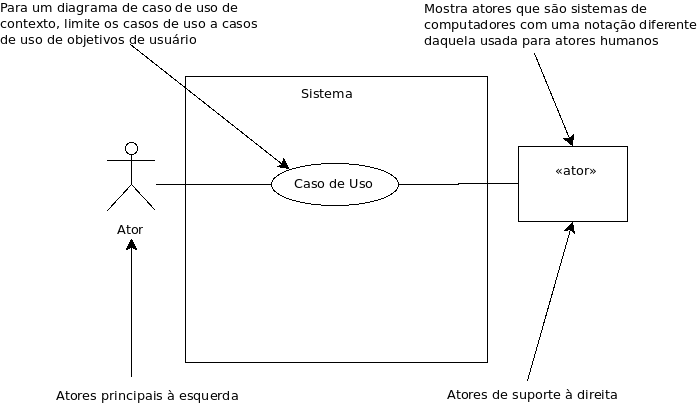
\includegraphics[scale=0.75]{images/exemplo-uml.png}
	\caption{Sugestões de notação de caso de uso proposto por ~\cite{larman08}}
	\label{fig:diagrama-uml}
\end{figure}

\paragraph{Diagrama de Sequência}
O Diagrama de Sequência é um documento criado para ilustrar os eventos descritos em um caso de uso de forma sequencial e temporal, mostrando a interação de atores externos ao sistema e os eventos que eles geram durante essa interação. A UML possui uma notação específica para este diagrama, onde todos os elementos são representados.

Neste diagrama, são representados para cada cenário do caso de uso os eventos que os atores geram, bem como a ordem da sua interação. No diagrama os atores são representados na parte superior (com a mesma notação do diagrama de caso de uso). Abaixo dos atores é apresentada a linha de tempo, crescendo de cima para baixo. 

Durante a interação do ator com o sistema, eventos de sistema são gerados e iniciam toda a execução do cenário do caso de uso, ou operação do sistema. A execução dos eventos ocorre até o último evento cronológico na linha do tempo. Os eventos gerados pela interação entre os atores ocorrem na linha do tempo de forma cronológica e ordenada com a mesma ordem dos eventos do cenário do caso de uso.

A nomenclatura dos eventos deve sempre iniciar com um verbo, podendo ser seguida de um substantivo. Além disso, deve-se sempre expressar a nomenclatura em níveis genéricos verbais, nunca detalhando a funcionalidade do sistema.

Na ilustração da notação de diagramas de sequência~\ref{fig:exemplo-diagrama-sequencia} é possível identificar a interação entre um ator e uma entidade do sistema. É fácil identificar que os eventos estão ocorrendo de forma ordenada de cima para baixo.
\begin{figure}
	\centering
	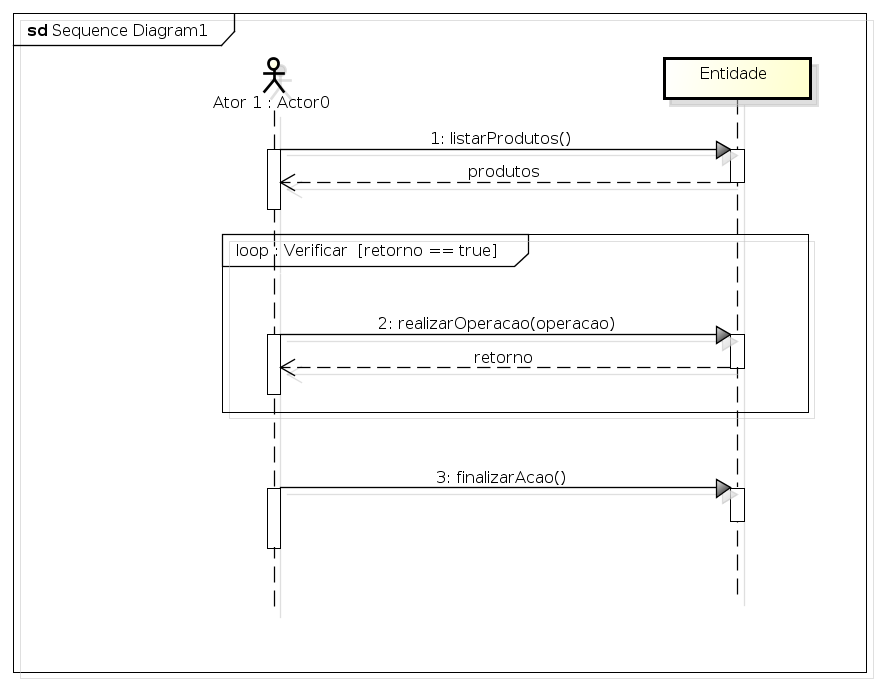
\includegraphics[scale=0.75]{images/exemplo-diagrama-sequencia.png}
	\caption{Notação de diagrama de sequência, exibindo a comunicação de um ator e uma entidade (sistema)}
	\label{fig:exemplo-diagrama-sequencia}
\end{figure}

O primeiro evento é iniciado pelo ator, onde o método~\emph(listarProdutos()) da Entidade é invocado. Esse método gera a resposta ~\emph(produtos) para o ator. A interação seguinte acontece dentro de um retângulo, do tipo~\emph{loop} e de nome "Verificar". Esse retângulo permite que o diagrama de sequências represente um loop, onde todos os eventos serão repetidos enquanto a condição de guarda for verdadeira, no caso do exemplo, enquanto retorno for igual a~\emph{true}. O UML permite diversos operadores além do loop, como por exemplo a negação, a assertiva, o~\emph{break}, dentre outros.

Dentro do retângulo, o ator chama o método~\emph(realizarOperacao), enviado o parâmetro~\emph{operação}. A entidade retorna um valor, que será testado na guarda para a continuidade da conversação. Por fim, o ator chama o método~\emph{finalizarAcao} da entidade. Por não haver outra interação em seguida, o cenário é considerado como encerrado. 

A importância do desenho de um diagrama de sequência está no fato de detalhar os eventos do sistema que são gerados pela interação de atores externos, pois assim é possível ter uma análise comportamental do sistema com base nesses eventos. Neste nível de análise, é possível estudar e projetar o comportamento do sistema no nível de projetar o que ele faz, porém sem necessariamente explicar como o faz~\cite{larman08}.

O diagrama de sequência geralmente está relacionado com o caso de uso, primeiramente pelo fato de descrever um cenário de caso de uso, mas também pelo fato de o caso de uso conter todos os detalhes do cenário. Ele apenas deixará claro a interação entre os atores e os eventos derivados dessa interação.


\subsection{Java Agent Development Framework}

JADE é um~\emph{middleware} desenvolvido em 1988 pela Telecom Italia, posteriormente (2000) tornando-se em um projeto open source. Seu desenvolvimento de baixo acoplamento permite que seja possível integrar várias bibliotecas auxiliares (~\emph{addons}) para facilitar o desenvolvimento de aplicações.

Em~\cite{bellifemine07}, ele foi desenvolvido seguindo todas as especificações da FIPA, o que garante uma intercomunicação com outras plataformas. O JADE foi desenvolvido na linguagem JAVA, possibilitando o uso de diversas bibliotecas e frameworks desenvolvidos na linguagem.

O middleware provê várias funcionalidades básicas que abstraem e simplificam o desenvolvimento de aplicações, com o objetivo do desenvolvedor estar mais preocupado com o comportamento do agente do que com a infra estrutura da plataforma.

O sistema de mensagem no JADE funciona de forma assíncrona. Um agente não precisa estar necessariamente disponível para receber as mensagens, visto que elas são enfileiradas e processadas em ordem. Além disso, não é necessário que um agente tenha uma referência para outro agente a fim de comunicar-se.

A arquitetura de um SMA desenvolvido em JADE funciona de forma semelhante à rede P2P (\emph{Peer-to-Peer}), onde cada agente possui um nome único na plataforma - Agent ID (AID) - e é livre para entrar e sair a qualquer momento durante a execução. Uma plafatorma JADE possui normalmente os seguintes elementos:

\begin{itemize}
	\item Agent Management System (AMS) é o agente responsável por supervisionar toda a plataforma e criar um elo entre os agentes. Esse tipo de serviço é chamado de~\emph{white pages} e indexa todos os agentes da plataforma.
	\item Directory Facilitator (DF) é o agente responsável por registrar todos os serviços e prover a funcionalidade de busca para os agentes. Este tipo de serviço é chamado de~\emph{yellow pages}.
\end{itemize}

Os agentes executam em threads separadas garantindo o não compartilhamento de recursos para evitar condições de corrida. A plataforma é responsável também por manter o ciclo de vida dos agentes. Durante a criação dos agentes, eles são automaticamente registrados no serviço de~\emph{white pages}

A mobilidade de agentes entre máquinas também é feita de forma transparente pelo JADE. Em~\cite{bellifemine07}, a mobilidade do agente pode transportar o estado do agente (sob certas condições) entre processos e máquinas.

Uma das características mais importantes do~\emph{middleware} é o suporte nativo à ontologias e linguagens de comunicação FIPA. As ontologias podem ser modeladas (expressando ações, conceitos e predicados) de forma simples e clara, além de ser possível restringir as ontologias à determinados agentes que devem a conhecer.

\subsubsection{Arquitetura}

A representação~\ref{fig:arquitetura-jade} do ambiente de execução JADE ilustra os principais elementos da arquitetura distribuídos em três máquinas (dois servidores e um~\emph{desktop}). Cada máquina possui um container e vários agentes.

\begin{figure}
	\centering
	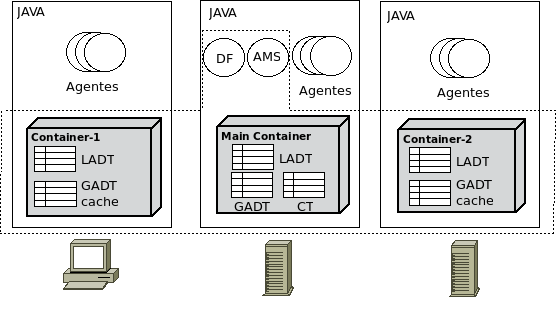
\includegraphics[scale=0.65]{images/arquitetura-jade.png}
	\caption{Representação da arquitetura principal do JADE.Adaptado de~\cite{bellifemine07}.}
	\label{fig:arquitetura-jade}
\end{figure}

O container principal(\emph{main container}), presente na máquina do centro, possui algumas diferenças entre os outros, chamados de~\emph{Container-1} e~\emph{Container-2}, abringando agentes primordiais na plataforma que atendem às especificações da FIPA (número 23 e 61~\cite{bellifemineGuide02}). O container principal possui o componente~\emph{container table} (CT), que possui as referências para os objetos e os endereços de comunicação dos nós que compõe a plataforma.

Além disso, o container principal possui uma tabela global para descrição de agentes (GADT) que registra todos os agentes da plataforma e o seu endereço. Os outros containeres possuem uma cópia em cache da tabela para, caso a tabela principal seja corrompida, possa ser substituída.

O primeiro deles é o~\emph{Directory Facilitator} (DF), agente responsável por registrar todos os serviços disponíveis na plataforma. O segundo agente é o~\emph{Agent Management System} (AMS) é o agente responsável por supervisionar toda a plataforma, registrando os agentes que estão rodando, bem como o seu estado. 

\subsubsection{Implementação dos Agentes}
O JADE define a classe abstrata~\emph{Agent}, que é a base para todos os agentes definidos. O desenvolvedor tem apenas o trabalho de extender esta classe e implementar o comportamento no método~\emph{setup()}. O fato de extender a classe abstrata implica em herdar várias características já definidas pelo JADE (registro, configuração, etc.) e métodos que podem ser chamados para a implementação do comportamento do agente.

Cada agente possui um identificador único (Agent ID - AID) que identifica o agente em toda plataforma. Por padrão, o formato do AID possui primeiramente o nome do agente seguido do caracter '@', por fim o endereço da plataforma onde o agente está. Este AID é atribuído durante o registro do agente no AMS. Neste registro, é possível também registrar os serviços do agente no DF.

Conforme dito anteriormente, o método~\emph{setup()} deverá ser implementado e, no mínimo, deverá ser estabelecido um comportamento para o agente. Este comportamento diz respeito à ação que será realizada pelo agente durante a ocorrência de um evento. O registro/cancelamento dos comportamentos é feito pelos métodos exibidos no trecho~\ref{code:exemplo-register}.

\begin{lstlisting}[language=java,label=code:exemplo-register,caption=Exemplo de registro de comportamento nos agentes.]
	void addBehaviour( Comportamento )
	void removeBehaviour( Comportamento )
	void addSubBehaviour( Comportamento )
	void removeSubBehaviour( Comportamento )
\end{lstlisting}

Os comportamentos são separados em primitivos e compostos. A diferença entre ambos é a possibilidade dos comportamentos compostos poderem agregar vários outros comportamentos simples ou compostos, sendo eles:~\emph{ParallelBehaviour, SequentialBehaviour}. De maneira distinta, os comportamentos primitivos tem relação direta com o tempo, acontecendo durante um período de espera ou após o envio de uma mensagem. São eles:~\emph{SimpleBehaviour, CyclicBehaviour, TickerBehaviour, OneShotBehaviour, WakerBehaviour} e~\emph{ReceiverBehaviour}.

\subsubsection{Ciclo de Vida dos Agentes}
O JADE implementa o ciclo de vida especificado pela FIPA. Os possíveis estados da plataforma são:

\begin{itemize}
	\item INITIATED - Após a criação do objeto, antes do registro do objeto no AMS, o agente assume o estado de iniciado. Este estado significa que o agente ainda não está disponível para a execução de ações na  plataforma.
	\item ACTIVE - Neste estado o agente é registrado no AMS, possuindo assim o AID e o endereço. Ele está pronto para a execução do trabalho na plataforma.
	\item SUSPENDED - O agente está com as atividades suspensas e está em modo ocioso.
	\item WAITING - O agente está bloqueado esperando algum evento acontecer para executar alguma ação. Tipicamente, este estado é usado para fazer o agente esperar por alguma mensagem.
	\item DELETED - O agente está destruído e sua thread de execução é terminada. O seu registro será removido do AMS e a sua referência removida da JVM.
	\item TRANSIT - O agente está movendo-se de uma plataforma para uma nova localização. Mesmo em transito, é possível enviar mensagens para este agente, visto que serão empilhadas na sua fila de mensagens e posteriormente processadas quando ele assumir o estado ACTIVE.
\end{itemize}

Para cada uma das transições de estados existem métodos que são invocados em um momento anterior. Eles são úteis para a execução de ações que antecedem a mudança de estado. Por exemplo: Durante a mudança do estado ACTIVE para DELETE, o método~\emph{doDelete()} é encarregado de implementar ações que antecedam o fim do agente, como que o agente desfaça o registro dos seus serviços no DF.

\subsubsection{Interface Gráfica}
O JADE permite o desenvolvimento de agentes com suporte à interface gráfica. Dessa forma, é possível desenvolver uma interação simples do agente com o ser humano.


Por padrão, o JADE utiliza diversos agentes que utilizam-se de interfaces gráficas para a comunicação dos humanos que, dentre outras funcionalidades, permitem o envio de dados, controle do agente e testes da plataforma. Ferramentas como gerência dos~\emph{containers}, visualização do DF, criação de mensagens a partir de agentes falsos (\emph{sniffers}), dentre outros são disponibilizados nativamente para o desenvolvedor.

Na representação básica do exemplo do agente RMA~\ref{fig:tela-jade}, é apresentada sua interface gráfica com o ambiente de execução em tempo real. É possível identificar apenas o~\emph{container} principal da aplicação. Nele, existem os três agentes principais registrados descritos anteriormente: AMS, DF e o próprio RMA.
\begin{figure}
	\centering
	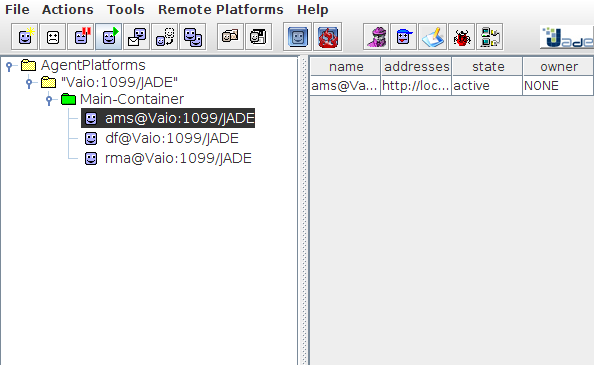
\includegraphics[scale=0.65]{images/tela-jade.png}
	\caption{Apresentação da Interface do agente RMA}
	\label{fig:tela-jade}
\end{figure}

\subsection{JBoss Seam}

No mundo corporativo do JAVA, muitos frameworks são responsáveis por partes específicas de uma aplicação. Seguindo as especificações propostas para a plataforma (JSR), as aplicações implementam integrações com o banco de dados (Hibernate, JPA), integração com a camada de visualização (Struts 1~\cite{struts1} e 2~\cite{struts2}, JSF~\cite{jsf2012}), contextos Java e injeção de dependência~\cite{di2012}. Porém a integração destes frameworks nem sempre é trivial, demandando muito tempo dos desenvolvedores para a correta configuração.

Neste aspecto surge o JBoss Seam. Ele é um~\emph{framework} que reune as principais tecnologias de desenvolvimento web na linguagem Java. Ele integra as tecnologias~\emph{Asynchronous JavaScript and XML} (AJAX),~\emph{JavaServer Faces} (JSF),~\emph{Java Persistence} (JPA),~\emph{Enterprise Java Beans} (EJB 3.0) e~\emph{Business Process Management} (BPM) em uma única ferramenta que objetiva o desenvolvimento ágil de aplicações e o foco do programador na lógica de negócio~\cite{seamSite}.

A pilha de aplicações do Seam~\ref{fig:servidor-app-seam} são todos as tecnologias que são utilizados pelo JBoss Seam. Caso o desenvolvedor deseje utilizar outras tecnologias, o Seam provê configurações para que outras ferramentas possam ser integradas facilmente à aplicação.

\begin{figure}
	\centering
	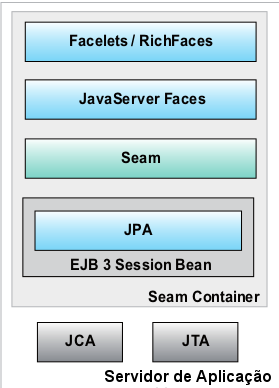
\includegraphics[scale=0.65]{images/servidor-app-seam.png}
	\caption{Representação da pilha de aplicações do Seam.~\cite{allen09}}
	\label{fig:servidor-app-seam}
\end{figure}

Em~\cite{allen09}, uma das principais ferramentas do Seam é o~\emph{seam-generator}. Com ele, é possível gerar uma estrutura básica de projeto, com arquivos de construção, bibliotecas compatíveis e as configurações necessárias para o início do desenvolvimento e o~\emph{deploy} em um servidor de aplicação.

Além disso, uma das grandes vantagens do~\emph{seam-generator} é a geração automática de código, criando a partir de uma tabela no banco de dados todas as operações necessárias para a visualização, inserção, exclusão e atualização de dados (CRUD), diminuindo assim o tempo de desenvolvimento de aplicações.

\section{Trabalhos Correlatos}
É possível fazer comparações deste trabalho com diversas áreas de conhecimentos correlatos. Os trabalhos presentes nesta seção foram selecionados a partir de um levantamento que buscou soluções para melhorias na educação com o apoio de tecnologia. Estes trabalhos estão relacionados com a área de atuação deste trabalho, seja em Inteligência Artificial, Estilos de Aprendizagem, Sistemas Multiagentes ou Ambientes Virtuais de Aprendizagem.

Na área de auxílio de alunos, alguns trabalhos assemelham-se com o propósito deste trabalho. A implementação de um agente artificial integrado à um tutor inteligente~\cite{soaresagente} que identifica dificuldades de aprendizagem por meio de técnicas de Inteligência Artificial. Ele prima pela agradável interação com humanos com o intuito de facilitar a compreensão da ferramenta. Sua abordagem porém não é voltada para a abordagem multidimensional de inferência do aluno, bem como a solução não prevê a inferência de dados vindos de outros Ambientes Virtuais de Aprendizagem.

Existem trabalhos na área de identificação de conhecimentos~\cite{bativa2011}, que visam a determinação de estilos de aprendizagem dos alunos por meio da plataforma chamada "Ferramenta de Identificação de Perfis de Aprendizes – FIPA", uma aplicação multicamadas que faz a identificação do perfil é feita por meio de questionários de estilos de aprendizagem. Apesar da inferência do estilo de aprendizagem, esta plataforma utiliza uma abordagem distinta deste trabalho, sendo uma arquitetura cliente-servidor.
 
O trabalho~\cite{geyer2001semeai} utiliza-se de Sistemas Multiagentes para a adaptação do ensino na internet. A adaptação ocorre conforme as características individuais de cada aluno e pode modificar características como a estratégia de ensino, seleção de materiais que são mais adequados ao aluno de acordo com o seu perfil. Este ambiente assemelha-se bastante com o presente trabalho, porém o seu foco não é na modelagem multidimensional do aluno.

Por fim, o Ambiente Virtual de Aprendizagem EDULIVRE~\cite{rabelo2010identificacao} constitui-se de um Ambiente Virtual de Aprendizagem que possibilita a inferência implícita de modelos e perfis individuais de estudantes da educação infantil. Com o perfil de cada aluno e de todos os alunos em geral, o educando poderá desenvolver nortear seu trabalho da melhor forma possível. A abordagem deste trabalho não é com uso de agentes, diferindo assim do foco deste trabalho. Além disso, o EDULIVRE apresenta a estratégia de ser o Ambiente Virtual de Aprendizagem e não permite integração com outros ambientes.















